% Created by tikzDevice version 0.12.6 on 2024-07-02 14:24:28
% !TEX encoding = UTF-8 Unicode
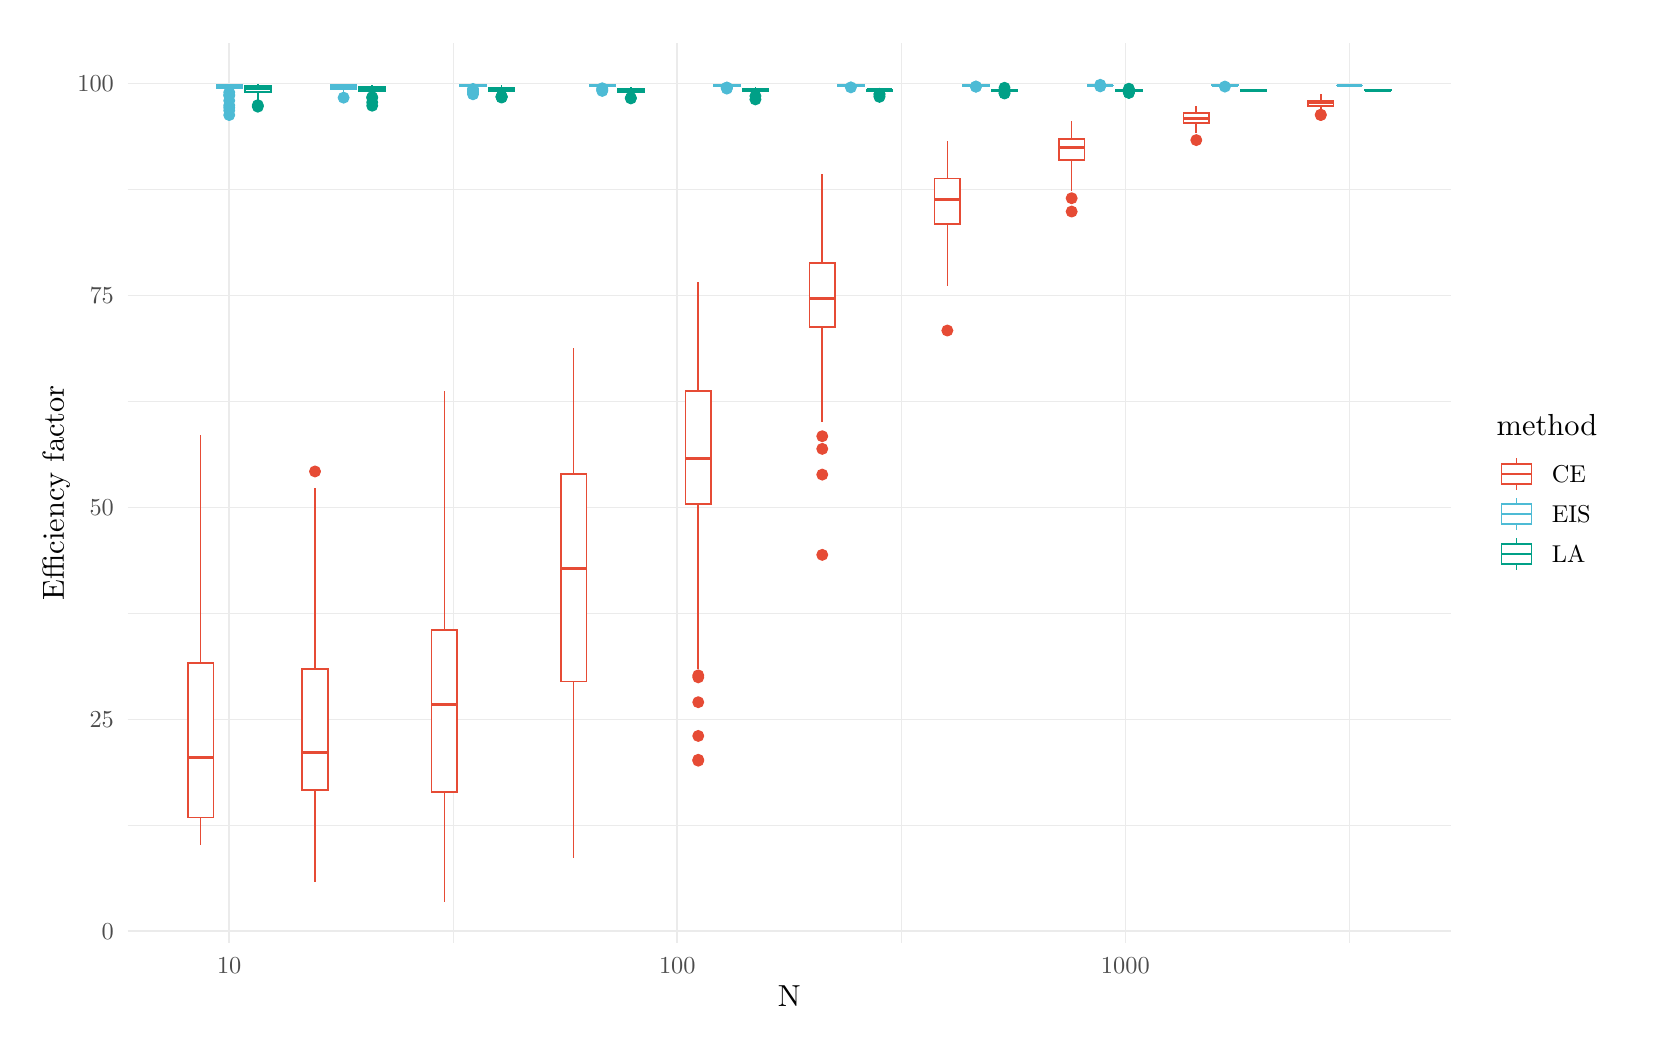
\begin{tikzpicture}[x=1pt,y=1pt]
\definecolor{fillColor}{RGB}{255,255,255}
\path[use as bounding box,fill=fillColor,fill opacity=0.00] (0,0) rectangle (578.16,361.35);
\begin{scope}
\path[clip] ( 36.11, 30.69) rectangle (514.31,355.85);
\definecolor{drawColor}{gray}{0.92}

\path[draw=drawColor,line width= 0.3pt,line join=round] ( 36.11, 73.12) --
	(514.31, 73.12);

\path[draw=drawColor,line width= 0.3pt,line join=round] ( 36.11,149.70) --
	(514.31,149.70);

\path[draw=drawColor,line width= 0.3pt,line join=round] ( 36.11,226.28) --
	(514.31,226.28);

\path[draw=drawColor,line width= 0.3pt,line join=round] ( 36.11,302.87) --
	(514.31,302.87);

\path[draw=drawColor,line width= 0.3pt,line join=round] (153.78, 30.69) --
	(153.78,355.85);

\path[draw=drawColor,line width= 0.3pt,line join=round] (315.69, 30.69) --
	(315.69,355.85);

\path[draw=drawColor,line width= 0.3pt,line join=round] (477.60, 30.69) --
	(477.60,355.85);

\path[draw=drawColor,line width= 0.6pt,line join=round] ( 36.11, 34.83) --
	(514.31, 34.83);

\path[draw=drawColor,line width= 0.6pt,line join=round] ( 36.11,111.41) --
	(514.31,111.41);

\path[draw=drawColor,line width= 0.6pt,line join=round] ( 36.11,187.99) --
	(514.31,187.99);

\path[draw=drawColor,line width= 0.6pt,line join=round] ( 36.11,264.58) --
	(514.31,264.58);

\path[draw=drawColor,line width= 0.6pt,line join=round] ( 36.11,341.16) --
	(514.31,341.16);

\path[draw=drawColor,line width= 0.6pt,line join=round] ( 72.83, 30.69) --
	( 72.83,355.85);

\path[draw=drawColor,line width= 0.6pt,line join=round] (234.74, 30.69) --
	(234.74,355.85);

\path[draw=drawColor,line width= 0.6pt,line join=round] (396.64, 30.69) --
	(396.64,355.85);
\definecolor{drawColor}{RGB}{230,75,53}

\path[draw=drawColor,line width= 0.6pt,line join=round] ( 62.50,131.76) -- ( 62.50,214.18);

\path[draw=drawColor,line width= 0.6pt,line join=round] ( 62.50, 75.95) -- ( 62.50, 66.00);
\definecolor{fillColor}{RGB}{255,255,255}

\path[draw=drawColor,line width= 0.6pt,fill=fillColor] ( 57.85,131.76) --
	( 57.85, 75.95) --
	( 67.15, 75.95) --
	( 67.15,131.76) --
	( 57.85,131.76) --
	cycle;

\path[draw=drawColor,line width= 1.1pt] ( 57.85, 97.75) -- ( 67.15, 97.75);
\definecolor{fillColor}{RGB}{230,75,53}

\path[draw=drawColor,line width= 0.4pt,line join=round,line cap=round,fill=fillColor] (103.83,200.99) circle (  1.96);

\path[draw=drawColor,line width= 0.6pt,line join=round] (103.83,129.53) -- (103.83,194.90);

\path[draw=drawColor,line width= 0.6pt,line join=round] (103.83, 85.90) -- (103.83, 52.59);
\definecolor{fillColor}{RGB}{255,255,255}

\path[draw=drawColor,line width= 0.6pt,fill=fillColor] ( 99.18,129.53) --
	( 99.18, 85.90) --
	(108.48, 85.90) --
	(108.48,129.53) --
	( 99.18,129.53) --
	cycle;

\path[draw=drawColor,line width= 1.1pt] ( 99.18, 99.40) -- (108.48, 99.40);

\path[draw=drawColor,line width= 0.6pt,line join=round] (150.59,143.64) -- (150.59,230.09);

\path[draw=drawColor,line width= 0.6pt,line join=round] (150.59, 85.25) -- (150.59, 45.47);

\path[draw=drawColor,line width= 0.6pt,fill=fillColor] (145.94,143.64) --
	(145.94, 85.25) --
	(155.23, 85.25) --
	(155.23,143.64) --
	(145.94,143.64) --
	cycle;

\path[draw=drawColor,line width= 1.1pt] (145.94,116.63) -- (155.23,116.63);

\path[draw=drawColor,line width= 0.6pt,line join=round] (197.29,200.07) -- (197.29,245.76);

\path[draw=drawColor,line width= 0.6pt,line join=round] (197.29,125.05) -- (197.29, 61.37);

\path[draw=drawColor,line width= 0.6pt,fill=fillColor] (192.64,200.07) --
	(192.64,125.05) --
	(201.94,125.05) --
	(201.94,200.07) --
	(192.64,200.07) --
	cycle;

\path[draw=drawColor,line width= 1.1pt] (192.64,165.94) -- (201.94,165.94);
\definecolor{fillColor}{RGB}{230,75,53}

\path[draw=drawColor,line width= 0.4pt,line join=round,line cap=round,fill=fillColor] (242.31, 96.80) circle (  1.96);

\path[draw=drawColor,line width= 0.4pt,line join=round,line cap=round,fill=fillColor] (242.31,126.59) circle (  1.96);

\path[draw=drawColor,line width= 0.4pt,line join=round,line cap=round,fill=fillColor] (242.31,127.30) circle (  1.96);

\path[draw=drawColor,line width= 0.4pt,line join=round,line cap=round,fill=fillColor] (242.31,117.61) circle (  1.96);

\path[draw=drawColor,line width= 0.4pt,line join=round,line cap=round,fill=fillColor] (242.31,105.42) circle (  1.96);

\path[draw=drawColor,line width= 0.4pt,line join=round,line cap=round,fill=fillColor] (242.31, 96.48) circle (  1.96);

\path[draw=drawColor,line width= 0.6pt,line join=round] (242.31,230.13) -- (242.31,269.57);

\path[draw=drawColor,line width= 0.6pt,line join=round] (242.31,189.13) -- (242.31,129.61);
\definecolor{fillColor}{RGB}{255,255,255}

\path[draw=drawColor,line width= 0.6pt,fill=fillColor] (237.66,230.13) --
	(237.66,189.13) --
	(246.96,189.13) --
	(246.96,230.13) --
	(237.66,230.13) --
	cycle;

\path[draw=drawColor,line width= 1.1pt] (237.66,205.78) -- (246.96,205.78);
\definecolor{fillColor}{RGB}{230,75,53}

\path[draw=drawColor,line width= 0.4pt,line join=round,line cap=round,fill=fillColor] (287.12,213.72) circle (  1.96);

\path[draw=drawColor,line width= 0.4pt,line join=round,line cap=round,fill=fillColor] (287.12,199.85) circle (  1.96);

\path[draw=drawColor,line width= 0.4pt,line join=round,line cap=round,fill=fillColor] (287.12,209.15) circle (  1.96);

\path[draw=drawColor,line width= 0.4pt,line join=round,line cap=round,fill=fillColor] (287.12,170.85) circle (  1.96);

\path[draw=drawColor,line width= 0.6pt,line join=round] (287.12,276.36) -- (287.12,308.57);

\path[draw=drawColor,line width= 0.6pt,line join=round] (287.12,253.18) -- (287.12,218.82);
\definecolor{fillColor}{RGB}{255,255,255}

\path[draw=drawColor,line width= 0.6pt,fill=fillColor] (282.47,276.36) --
	(282.47,253.18) --
	(291.77,253.18) --
	(291.77,276.36) --
	(282.47,276.36) --
	cycle;

\path[draw=drawColor,line width= 1.1pt] (282.47,263.56) -- (291.77,263.56);
\definecolor{fillColor}{RGB}{230,75,53}

\path[draw=drawColor,line width= 0.4pt,line join=round,line cap=round,fill=fillColor] (332.32,251.91) circle (  1.96);

\path[draw=drawColor,line width= 0.6pt,line join=round] (332.32,306.80) -- (332.32,320.32);

\path[draw=drawColor,line width= 0.6pt,line join=round] (332.32,290.41) -- (332.32,268.14);
\definecolor{fillColor}{RGB}{255,255,255}

\path[draw=drawColor,line width= 0.6pt,fill=fillColor] (327.67,306.80) --
	(327.67,290.41) --
	(336.97,290.41) --
	(336.97,306.80) --
	(327.67,306.80) --
	cycle;

\path[draw=drawColor,line width= 1.1pt] (327.67,299.37) -- (336.97,299.37);
\definecolor{fillColor}{RGB}{230,75,53}

\path[draw=drawColor,line width= 0.4pt,line join=round,line cap=round,fill=fillColor] (377.24,299.72) circle (  1.96);

\path[draw=drawColor,line width= 0.4pt,line join=round,line cap=round,fill=fillColor] (377.24,294.90) circle (  1.96);

\path[draw=drawColor,line width= 0.6pt,line join=round] (377.24,321.10) -- (377.24,327.76);

\path[draw=drawColor,line width= 0.6pt,line join=round] (377.24,313.59) -- (377.24,302.41);
\definecolor{fillColor}{RGB}{255,255,255}

\path[draw=drawColor,line width= 0.6pt,fill=fillColor] (372.59,321.10) --
	(372.59,313.59) --
	(381.89,313.59) --
	(381.89,321.10) --
	(372.59,321.10) --
	cycle;

\path[draw=drawColor,line width= 1.1pt] (372.59,318.09) -- (381.89,318.09);
\definecolor{fillColor}{RGB}{230,75,53}

\path[draw=drawColor,line width= 0.4pt,line join=round,line cap=round,fill=fillColor] (422.28,320.72) circle (  1.96);

\path[draw=drawColor,line width= 0.6pt,line join=round] (422.28,330.41) -- (422.28,332.91);

\path[draw=drawColor,line width= 0.6pt,line join=round] (422.28,327.01) -- (422.28,323.45);
\definecolor{fillColor}{RGB}{255,255,255}

\path[draw=drawColor,line width= 0.6pt,fill=fillColor] (417.63,330.41) --
	(417.63,327.01) --
	(426.93,327.01) --
	(426.93,330.41) --
	(417.63,330.41) --
	cycle;

\path[draw=drawColor,line width= 1.1pt] (417.63,328.59) -- (426.93,328.59);
\definecolor{fillColor}{RGB}{230,75,53}

\path[draw=drawColor,line width= 0.4pt,line join=round,line cap=round,fill=fillColor] (467.26,329.90) circle (  1.96);

\path[draw=drawColor,line width= 0.4pt,line join=round,line cap=round,fill=fillColor] (467.26,329.77) circle (  1.96);

\path[draw=drawColor,line width= 0.6pt,line join=round] (467.26,335.04) -- (467.26,337.21);

\path[draw=drawColor,line width= 0.6pt,line join=round] (467.26,333.13) -- (467.26,330.88);
\definecolor{fillColor}{RGB}{255,255,255}

\path[draw=drawColor,line width= 0.6pt,fill=fillColor] (462.61,335.04) --
	(462.61,333.13) --
	(471.91,333.13) --
	(471.91,335.04) --
	(462.61,335.04) --
	cycle;

\path[draw=drawColor,line width= 1.1pt] (462.61,334.20) -- (471.91,334.20);
\definecolor{drawColor}{RGB}{77,187,213}
\definecolor{fillColor}{RGB}{77,187,213}

\path[draw=drawColor,line width= 0.4pt,line join=round,line cap=round,fill=fillColor] ( 72.83,329.77) circle (  1.96);

\path[draw=drawColor,line width= 0.4pt,line join=round,line cap=round,fill=fillColor] ( 72.83,337.99) circle (  1.96);

\path[draw=drawColor,line width= 0.4pt,line join=round,line cap=round,fill=fillColor] ( 72.83,334.99) circle (  1.96);

\path[draw=drawColor,line width= 0.4pt,line join=round,line cap=round,fill=fillColor] ( 72.83,331.41) circle (  1.96);

\path[draw=drawColor,line width= 0.4pt,line join=round,line cap=round,fill=fillColor] ( 72.83,337.08) circle (  1.96);

\path[draw=drawColor,line width= 0.4pt,line join=round,line cap=round,fill=fillColor] ( 72.83,333.29) circle (  1.96);

\path[draw=drawColor,line width= 0.4pt,line join=round,line cap=round,fill=fillColor] ( 72.83,332.48) circle (  1.96);

\path[draw=drawColor,line width= 0.4pt,line join=round,line cap=round,fill=fillColor] ( 72.83,336.76) circle (  1.96);

\path[draw=drawColor,line width= 0.6pt,line join=round] ( 72.83,340.64) -- ( 72.83,341.07);

\path[draw=drawColor,line width= 0.6pt,line join=round] ( 72.83,339.60) -- ( 72.83,338.18);
\definecolor{fillColor}{RGB}{255,255,255}

\path[draw=drawColor,line width= 0.6pt,fill=fillColor] ( 68.18,340.64) --
	( 68.18,339.60) --
	( 77.48,339.60) --
	( 77.48,340.64) --
	( 68.18,340.64) --
	cycle;

\path[draw=drawColor,line width= 1.1pt] ( 68.18,340.28) -- ( 77.48,340.28);
\definecolor{fillColor}{RGB}{77,187,213}

\path[draw=drawColor,line width= 0.4pt,line join=round,line cap=round,fill=fillColor] (114.16,336.05) circle (  1.96);

\path[draw=drawColor,line width= 0.6pt,line join=round] (114.16,340.59) -- (114.16,341.04);

\path[draw=drawColor,line width= 0.6pt,line join=round] (114.16,339.20) -- (114.16,337.34);
\definecolor{fillColor}{RGB}{255,255,255}

\path[draw=drawColor,line width= 0.6pt,fill=fillColor] (109.51,340.59) --
	(109.51,339.20) --
	(118.81,339.20) --
	(118.81,340.59) --
	(109.51,340.59) --
	cycle;

\path[draw=drawColor,line width= 1.1pt] (109.51,340.21) -- (118.81,340.21);
\definecolor{fillColor}{RGB}{77,187,213}

\path[draw=drawColor,line width= 0.4pt,line join=round,line cap=round,fill=fillColor] (160.92,338.16) circle (  1.96);

\path[draw=drawColor,line width= 0.4pt,line join=round,line cap=round,fill=fillColor] (160.92,337.88) circle (  1.96);

\path[draw=drawColor,line width= 0.4pt,line join=round,line cap=round,fill=fillColor] (160.92,337.27) circle (  1.96);

\path[draw=drawColor,line width= 0.4pt,line join=round,line cap=round,fill=fillColor] (160.92,339.21) circle (  1.96);

\path[draw=drawColor,line width= 0.4pt,line join=round,line cap=round,fill=fillColor] (160.92,338.82) circle (  1.96);

\path[draw=drawColor,line width= 0.6pt,line join=round] (160.92,340.61) -- (160.92,341.03);

\path[draw=drawColor,line width= 0.6pt,line join=round] (160.92,340.08) -- (160.92,339.32);
\definecolor{fillColor}{RGB}{255,255,255}

\path[draw=drawColor,line width= 0.6pt,fill=fillColor] (156.27,340.61) --
	(156.27,340.08) --
	(165.57,340.08) --
	(165.57,340.61) --
	(156.27,340.61) --
	cycle;

\path[draw=drawColor,line width= 1.1pt] (156.27,340.38) -- (165.57,340.38);
\definecolor{fillColor}{RGB}{77,187,213}

\path[draw=drawColor,line width= 0.4pt,line join=round,line cap=round,fill=fillColor] (207.62,338.49) circle (  1.96);

\path[draw=drawColor,line width= 0.4pt,line join=round,line cap=round,fill=fillColor] (207.62,339.45) circle (  1.96);

\path[draw=drawColor,line width= 0.4pt,line join=round,line cap=round,fill=fillColor] (207.62,339.06) circle (  1.96);

\path[draw=drawColor,line width= 0.4pt,line join=round,line cap=round,fill=fillColor] (207.62,338.76) circle (  1.96);

\path[draw=drawColor,line width= 0.6pt,line join=round] (207.62,340.62) -- (207.62,340.88);

\path[draw=drawColor,line width= 0.6pt,line join=round] (207.62,340.21) -- (207.62,339.68);
\definecolor{fillColor}{RGB}{255,255,255}

\path[draw=drawColor,line width= 0.6pt,fill=fillColor] (202.97,340.62) --
	(202.97,340.21) --
	(212.27,340.21) --
	(212.27,340.62) --
	(202.97,340.62) --
	cycle;

\path[draw=drawColor,line width= 1.1pt] (202.97,340.41) -- (212.27,340.41);
\definecolor{fillColor}{RGB}{77,187,213}

\path[draw=drawColor,line width= 0.4pt,line join=round,line cap=round,fill=fillColor] (252.64,339.61) circle (  1.96);

\path[draw=drawColor,line width= 0.4pt,line join=round,line cap=round,fill=fillColor] (252.64,339.70) circle (  1.96);

\path[draw=drawColor,line width= 0.4pt,line join=round,line cap=round,fill=fillColor] (252.64,339.65) circle (  1.96);

\path[draw=drawColor,line width= 0.4pt,line join=round,line cap=round,fill=fillColor] (252.64,339.33) circle (  1.96);

\path[draw=drawColor,line width= 0.6pt,line join=round] (252.64,340.56) -- (252.64,340.80);

\path[draw=drawColor,line width= 0.6pt,line join=round] (252.64,340.23) -- (252.64,339.75);
\definecolor{fillColor}{RGB}{255,255,255}

\path[draw=drawColor,line width= 0.6pt,fill=fillColor] (247.99,340.56) --
	(247.99,340.23) --
	(257.29,340.23) --
	(257.29,340.56) --
	(247.99,340.56) --
	cycle;

\path[draw=drawColor,line width= 1.1pt] (247.99,340.44) -- (257.29,340.44);
\definecolor{fillColor}{RGB}{77,187,213}

\path[draw=drawColor,line width= 0.4pt,line join=round,line cap=round,fill=fillColor] (297.46,339.78) circle (  1.96);

\path[draw=drawColor,line width= 0.6pt,line join=round] (297.46,340.54) -- (297.46,340.76);

\path[draw=drawColor,line width= 0.6pt,line join=round] (297.46,340.30) -- (297.46,339.97);
\definecolor{fillColor}{RGB}{255,255,255}

\path[draw=drawColor,line width= 0.6pt,fill=fillColor] (292.81,340.54) --
	(292.81,340.30) --
	(302.11,340.30) --
	(302.11,340.54) --
	(292.81,340.54) --
	cycle;

\path[draw=drawColor,line width= 1.1pt] (292.81,340.43) -- (302.11,340.43);
\definecolor{fillColor}{RGB}{77,187,213}

\path[draw=drawColor,line width= 0.4pt,line join=round,line cap=round,fill=fillColor] (342.65,340.06) circle (  1.96);

\path[draw=drawColor,line width= 0.4pt,line join=round,line cap=round,fill=fillColor] (342.65,340.04) circle (  1.96);

\path[draw=drawColor,line width= 0.6pt,line join=round] (342.65,340.55) -- (342.65,340.67);

\path[draw=drawColor,line width= 0.6pt,line join=round] (342.65,340.37) -- (342.65,340.13);
\definecolor{fillColor}{RGB}{255,255,255}

\path[draw=drawColor,line width= 0.6pt,fill=fillColor] (338.00,340.55) --
	(338.00,340.37) --
	(347.30,340.37) --
	(347.30,340.55) --
	(338.00,340.55) --
	cycle;

\path[draw=drawColor,line width= 1.1pt] (338.00,340.47) -- (347.30,340.47);
\definecolor{fillColor}{RGB}{77,187,213}

\path[draw=drawColor,line width= 0.4pt,line join=round,line cap=round,fill=fillColor] (387.57,340.70) circle (  1.96);

\path[draw=drawColor,line width= 0.4pt,line join=round,line cap=round,fill=fillColor] (387.57,340.14) circle (  1.96);

\path[draw=drawColor,line width= 0.6pt,line join=round] (387.57,340.51) -- (387.57,340.64);

\path[draw=drawColor,line width= 0.6pt,line join=round] (387.57,340.39) -- (387.57,340.22);
\definecolor{fillColor}{RGB}{255,255,255}

\path[draw=drawColor,line width= 0.6pt,fill=fillColor] (382.92,340.51) --
	(382.92,340.39) --
	(392.22,340.39) --
	(392.22,340.51) --
	(382.92,340.51) --
	cycle;

\path[draw=drawColor,line width= 1.1pt] (382.92,340.46) -- (392.22,340.46);
\definecolor{fillColor}{RGB}{77,187,213}

\path[draw=drawColor,line width= 0.4pt,line join=round,line cap=round,fill=fillColor] (432.62,340.06) circle (  1.96);

\path[draw=drawColor,line width= 0.6pt,line join=round] (432.62,340.52) -- (432.62,340.58);

\path[draw=drawColor,line width= 0.6pt,line join=round] (432.62,340.42) -- (432.62,340.32);
\definecolor{fillColor}{RGB}{255,255,255}

\path[draw=drawColor,line width= 0.6pt,fill=fillColor] (427.97,340.52) --
	(427.97,340.42) --
	(437.27,340.42) --
	(437.27,340.52) --
	(427.97,340.52) --
	cycle;

\path[draw=drawColor,line width= 1.1pt] (427.97,340.46) -- (437.27,340.46);

\path[draw=drawColor,line width= 0.6pt,line join=round] (477.59,340.51) -- (477.59,340.58);

\path[draw=drawColor,line width= 0.6pt,line join=round] (477.59,340.44) -- (477.59,340.34);

\path[draw=drawColor,line width= 0.6pt,fill=fillColor] (472.94,340.51) --
	(472.94,340.44) --
	(482.24,340.44) --
	(482.24,340.51) --
	(472.94,340.51) --
	cycle;

\path[draw=drawColor,line width= 1.1pt] (472.94,340.48) -- (482.24,340.48);
\definecolor{drawColor}{RGB}{0,160,135}
\definecolor{fillColor}{RGB}{0,160,135}

\path[draw=drawColor,line width= 0.4pt,line join=round,line cap=round,fill=fillColor] ( 83.16,332.80) circle (  1.96);

\path[draw=drawColor,line width= 0.4pt,line join=round,line cap=round,fill=fillColor] ( 83.16,333.33) circle (  1.96);

\path[draw=drawColor,line width= 0.6pt,line join=round] ( 83.16,340.15) -- ( 83.16,340.85);

\path[draw=drawColor,line width= 0.6pt,line join=round] ( 83.16,338.09) -- ( 83.16,335.17);
\definecolor{fillColor}{RGB}{255,255,255}

\path[draw=drawColor,line width= 0.6pt,fill=fillColor] ( 78.51,340.15) --
	( 78.51,338.09) --
	( 87.81,338.09) --
	( 87.81,340.15) --
	( 78.51,340.15) --
	cycle;

\path[draw=drawColor,line width= 1.1pt] ( 78.51,339.42) -- ( 87.81,339.42);
\definecolor{fillColor}{RGB}{0,160,135}

\path[draw=drawColor,line width= 0.4pt,line join=round,line cap=round,fill=fillColor] (124.49,333.15) circle (  1.96);

\path[draw=drawColor,line width= 0.4pt,line join=round,line cap=round,fill=fillColor] (124.49,334.36) circle (  1.96);

\path[draw=drawColor,line width= 0.4pt,line join=round,line cap=round,fill=fillColor] (124.49,335.99) circle (  1.96);

\path[draw=drawColor,line width= 0.4pt,line join=round,line cap=round,fill=fillColor] (124.49,336.26) circle (  1.96);

\path[draw=drawColor,line width= 0.6pt,line join=round] (124.49,339.93) -- (124.49,340.70);

\path[draw=drawColor,line width= 0.6pt,line join=round] (124.49,338.56) -- (124.49,336.59);
\definecolor{fillColor}{RGB}{255,255,255}

\path[draw=drawColor,line width= 0.6pt,fill=fillColor] (119.84,339.93) --
	(119.84,338.56) --
	(129.14,338.56) --
	(129.14,339.93) --
	(119.84,339.93) --
	cycle;

\path[draw=drawColor,line width= 1.1pt] (119.84,339.27) -- (129.14,339.27);
\definecolor{fillColor}{RGB}{0,160,135}

\path[draw=drawColor,line width= 0.4pt,line join=round,line cap=round,fill=fillColor] (171.25,336.31) circle (  1.96);

\path[draw=drawColor,line width= 0.4pt,line join=round,line cap=round,fill=fillColor] (171.25,336.54) circle (  1.96);

\path[draw=drawColor,line width= 0.4pt,line join=round,line cap=round,fill=fillColor] (171.25,336.10) circle (  1.96);

\path[draw=drawColor,line width= 0.4pt,line join=round,line cap=round,fill=fillColor] (171.25,336.48) circle (  1.96);

\path[draw=drawColor,line width= 0.6pt,line join=round] (171.25,339.60) -- (171.25,340.53);

\path[draw=drawColor,line width= 0.6pt,line join=round] (171.25,338.38) -- (171.25,337.26);
\definecolor{fillColor}{RGB}{255,255,255}

\path[draw=drawColor,line width= 0.6pt,fill=fillColor] (166.60,339.60) --
	(166.60,338.38) --
	(175.90,338.38) --
	(175.90,339.60) --
	(166.60,339.60) --
	cycle;

\path[draw=drawColor,line width= 1.1pt] (166.60,338.91) -- (175.90,338.91);
\definecolor{fillColor}{RGB}{0,160,135}

\path[draw=drawColor,line width= 0.4pt,line join=round,line cap=round,fill=fillColor] (217.95,336.00) circle (  1.96);

\path[draw=drawColor,line width= 0.4pt,line join=round,line cap=round,fill=fillColor] (217.95,335.79) circle (  1.96);

\path[draw=drawColor,line width= 0.6pt,line join=round] (217.95,339.10) -- (217.95,340.08);

\path[draw=drawColor,line width= 0.6pt,line join=round] (217.95,337.98) -- (217.95,336.72);
\definecolor{fillColor}{RGB}{255,255,255}

\path[draw=drawColor,line width= 0.6pt,fill=fillColor] (213.30,339.10) --
	(213.30,337.98) --
	(222.60,337.98) --
	(222.60,339.10) --
	(213.30,339.10) --
	cycle;

\path[draw=drawColor,line width= 1.1pt] (213.30,338.74) -- (222.60,338.74);
\definecolor{fillColor}{RGB}{0,160,135}

\path[draw=drawColor,line width= 0.4pt,line join=round,line cap=round,fill=fillColor] (262.97,335.42) circle (  1.96);

\path[draw=drawColor,line width= 0.4pt,line join=round,line cap=round,fill=fillColor] (262.97,336.66) circle (  1.96);

\path[draw=drawColor,line width= 0.6pt,line join=round] (262.97,339.10) -- (262.97,340.06);

\path[draw=drawColor,line width= 0.6pt,line join=round] (262.97,338.24) -- (262.97,337.01);
\definecolor{fillColor}{RGB}{255,255,255}

\path[draw=drawColor,line width= 0.6pt,fill=fillColor] (258.32,339.10) --
	(258.32,338.24) --
	(267.62,338.24) --
	(267.62,339.10) --
	(258.32,339.10) --
	cycle;

\path[draw=drawColor,line width= 1.1pt] (258.32,338.73) -- (267.62,338.73);
\definecolor{fillColor}{RGB}{0,160,135}

\path[draw=drawColor,line width= 0.4pt,line join=round,line cap=round,fill=fillColor] (307.79,336.34) circle (  1.96);

\path[draw=drawColor,line width= 0.4pt,line join=round,line cap=round,fill=fillColor] (307.79,336.62) circle (  1.96);

\path[draw=drawColor,line width= 0.4pt,line join=round,line cap=round,fill=fillColor] (307.79,337.43) circle (  1.96);

\path[draw=drawColor,line width= 0.4pt,line join=round,line cap=round,fill=fillColor] (307.79,337.31) circle (  1.96);

\path[draw=drawColor,line width= 0.6pt,line join=round] (307.79,339.04) -- (307.79,339.71);

\path[draw=drawColor,line width= 0.6pt,line join=round] (307.79,338.40) -- (307.79,337.76);
\definecolor{fillColor}{RGB}{255,255,255}

\path[draw=drawColor,line width= 0.6pt,fill=fillColor] (303.14,339.04) --
	(303.14,338.40) --
	(312.44,338.40) --
	(312.44,339.04) --
	(303.14,339.04) --
	cycle;

\path[draw=drawColor,line width= 1.1pt] (303.14,338.82) -- (312.44,338.82);
\definecolor{fillColor}{RGB}{0,160,135}

\path[draw=drawColor,line width= 0.4pt,line join=round,line cap=round,fill=fillColor] (352.98,337.57) circle (  1.96);

\path[draw=drawColor,line width= 0.4pt,line join=round,line cap=round,fill=fillColor] (352.98,337.75) circle (  1.96);

\path[draw=drawColor,line width= 0.4pt,line join=round,line cap=round,fill=fillColor] (352.98,339.63) circle (  1.96);

\path[draw=drawColor,line width= 0.6pt,line join=round] (352.98,338.93) -- (352.98,339.37);

\path[draw=drawColor,line width= 0.6pt,line join=round] (352.98,338.50) -- (352.98,338.00);
\definecolor{fillColor}{RGB}{255,255,255}

\path[draw=drawColor,line width= 0.6pt,fill=fillColor] (348.33,338.93) --
	(348.33,338.50) --
	(357.63,338.50) --
	(357.63,338.93) --
	(348.33,338.93) --
	cycle;

\path[draw=drawColor,line width= 1.1pt] (348.33,338.75) -- (357.63,338.75);
\definecolor{fillColor}{RGB}{0,160,135}

\path[draw=drawColor,line width= 0.4pt,line join=round,line cap=round,fill=fillColor] (397.91,337.77) circle (  1.96);

\path[draw=drawColor,line width= 0.4pt,line join=round,line cap=round,fill=fillColor] (397.91,337.87) circle (  1.96);

\path[draw=drawColor,line width= 0.4pt,line join=round,line cap=round,fill=fillColor] (397.91,339.28) circle (  1.96);

\path[draw=drawColor,line width= 0.6pt,line join=round] (397.91,338.81) -- (397.91,339.09);

\path[draw=drawColor,line width= 0.6pt,line join=round] (397.91,338.50) -- (397.91,338.09);
\definecolor{fillColor}{RGB}{255,255,255}

\path[draw=drawColor,line width= 0.6pt,fill=fillColor] (393.26,338.81) --
	(393.26,338.50) --
	(402.56,338.50) --
	(402.56,338.81) --
	(393.26,338.81) --
	cycle;

\path[draw=drawColor,line width= 1.1pt] (393.26,338.71) -- (402.56,338.71);

\path[draw=drawColor,line width= 0.6pt,line join=round] (442.95,338.81) -- (442.95,339.13);

\path[draw=drawColor,line width= 0.6pt,line join=round] (442.95,338.54) -- (442.95,338.14);

\path[draw=drawColor,line width= 0.6pt,fill=fillColor] (438.30,338.81) --
	(438.30,338.54) --
	(447.60,338.54) --
	(447.60,338.81) --
	(438.30,338.81) --
	cycle;

\path[draw=drawColor,line width= 1.1pt] (438.30,338.68) -- (447.60,338.68);

\path[draw=drawColor,line width= 0.6pt,line join=round] (487.92,338.77) -- (487.92,339.02);

\path[draw=drawColor,line width= 0.6pt,line join=round] (487.92,338.60) -- (487.92,338.34);

\path[draw=drawColor,line width= 0.6pt,fill=fillColor] (483.27,338.77) --
	(483.27,338.60) --
	(492.57,338.60) --
	(492.57,338.77) --
	(483.27,338.77) --
	cycle;

\path[draw=drawColor,line width= 1.1pt] (483.27,338.68) -- (492.57,338.68);
\end{scope}
\begin{scope}
\path[clip] (  0.00,  0.00) rectangle (578.16,361.35);
\definecolor{drawColor}{gray}{0.30}

\node[text=drawColor,anchor=base east,inner sep=0pt, outer sep=0pt, scale=  0.88] at ( 31.16, 31.80) {0};

\node[text=drawColor,anchor=base east,inner sep=0pt, outer sep=0pt, scale=  0.88] at ( 31.16,108.38) {25};

\node[text=drawColor,anchor=base east,inner sep=0pt, outer sep=0pt, scale=  0.88] at ( 31.16,184.96) {50};

\node[text=drawColor,anchor=base east,inner sep=0pt, outer sep=0pt, scale=  0.88] at ( 31.16,261.55) {75};

\node[text=drawColor,anchor=base east,inner sep=0pt, outer sep=0pt, scale=  0.88] at ( 31.16,338.13) {100};
\end{scope}
\begin{scope}
\path[clip] (  0.00,  0.00) rectangle (578.16,361.35);
\definecolor{drawColor}{gray}{0.30}

\node[text=drawColor,anchor=base,inner sep=0pt, outer sep=0pt, scale=  0.88] at ( 72.83, 19.68) {10};

\node[text=drawColor,anchor=base,inner sep=0pt, outer sep=0pt, scale=  0.88] at (234.74, 19.68) {100};

\node[text=drawColor,anchor=base,inner sep=0pt, outer sep=0pt, scale=  0.88] at (396.64, 19.68) {1000};
\end{scope}
\begin{scope}
\path[clip] (  0.00,  0.00) rectangle (578.16,361.35);
\definecolor{drawColor}{RGB}{0,0,0}

\node[text=drawColor,anchor=base,inner sep=0pt, outer sep=0pt, scale=  1.10] at (275.21,  7.64) {N};
\end{scope}
\begin{scope}
\path[clip] (  0.00,  0.00) rectangle (578.16,361.35);
\definecolor{drawColor}{RGB}{0,0,0}

\node[text=drawColor,rotate= 90.00,anchor=base,inner sep=0pt, outer sep=0pt, scale=  1.10] at ( 13.08,193.27) {Efficiency factor};
\end{scope}
\begin{scope}
\path[clip] (  0.00,  0.00) rectangle (578.16,361.35);
\definecolor{drawColor}{RGB}{0,0,0}

\node[text=drawColor,anchor=base west,inner sep=0pt, outer sep=0pt, scale=  1.10] at (530.81,213.91) {method};
\end{scope}
\begin{scope}
\path[clip] (  0.00,  0.00) rectangle (578.16,361.35);
\definecolor{drawColor}{RGB}{230,75,53}

\path[draw=drawColor,line width= 0.6pt] (538.03,194.33) --
	(538.03,196.50);

\path[draw=drawColor,line width= 0.6pt] (538.03,203.73) --
	(538.03,205.90);
\definecolor{fillColor}{RGB}{255,255,255}

\path[draw=drawColor,line width= 0.6pt,fill=fillColor] (532.61,196.50) rectangle (543.45,203.73);

\path[draw=drawColor,line width= 0.6pt] (532.61,200.11) --
	(543.45,200.11);
\end{scope}
\begin{scope}
\path[clip] (  0.00,  0.00) rectangle (578.16,361.35);
\definecolor{drawColor}{RGB}{77,187,213}

\path[draw=drawColor,line width= 0.6pt] (538.03,179.88) --
	(538.03,182.05);

\path[draw=drawColor,line width= 0.6pt] (538.03,189.27) --
	(538.03,191.44);
\definecolor{fillColor}{RGB}{255,255,255}

\path[draw=drawColor,line width= 0.6pt,fill=fillColor] (532.61,182.05) rectangle (543.45,189.27);

\path[draw=drawColor,line width= 0.6pt] (532.61,185.66) --
	(543.45,185.66);
\end{scope}
\begin{scope}
\path[clip] (  0.00,  0.00) rectangle (578.16,361.35);
\definecolor{drawColor}{RGB}{0,160,135}

\path[draw=drawColor,line width= 0.6pt] (538.03,165.43) --
	(538.03,167.59);

\path[draw=drawColor,line width= 0.6pt] (538.03,174.82) --
	(538.03,176.99);
\definecolor{fillColor}{RGB}{255,255,255}

\path[draw=drawColor,line width= 0.6pt,fill=fillColor] (532.61,167.59) rectangle (543.45,174.82);

\path[draw=drawColor,line width= 0.6pt] (532.61,171.21) --
	(543.45,171.21);
\end{scope}
\begin{scope}
\path[clip] (  0.00,  0.00) rectangle (578.16,361.35);
\definecolor{drawColor}{RGB}{0,0,0}

\node[text=drawColor,anchor=base west,inner sep=0pt, outer sep=0pt, scale=  0.88] at (550.76,197.08) {CE};
\end{scope}
\begin{scope}
\path[clip] (  0.00,  0.00) rectangle (578.16,361.35);
\definecolor{drawColor}{RGB}{0,0,0}

\node[text=drawColor,anchor=base west,inner sep=0pt, outer sep=0pt, scale=  0.88] at (550.76,182.63) {EIS};
\end{scope}
\begin{scope}
\path[clip] (  0.00,  0.00) rectangle (578.16,361.35);
\definecolor{drawColor}{RGB}{0,0,0}

\node[text=drawColor,anchor=base west,inner sep=0pt, outer sep=0pt, scale=  0.88] at (550.76,168.18) {LA};
\end{scope}
\end{tikzpicture}
